\documentclass[10pt,landscape]{article}
\usepackage{multicol}
\usepackage{calc}
\usepackage{ifthen}
\usepackage[landscape]{geometry}
\usepackage{hyperref}
\usepackage{amsmath}
\usepackage{graphicx}

% To make this come out properly in landscape mode, do one of the following
% 1.
%  pdflatex latexsheet.tex
%
% 2.
%  latex latexsheet.tex
%  dvips -P pdf  -t landscape latexsheet.dvi
%  ps2pdf latexsheet.ps


% If you're reading this, be prepared for confusion.  Making this was
% a learning experience for me, and it shows.  Much of the placement
% was hacked in; if you make it better, let me know...


% 2008-04
% Changed page margin code to use the geometry package. Also added code for
% conditional page margins, depending on paper size. Thanks to Uwe Ziegenhagen
% for the suggestions.

% 2006-08
% Made changes based on suggestions from Gene Cooperman. <gene at ccs.neu.edu>


% To Do:
% \listoffigures \listoftables
% \setcounter{secnumdepth}{0}


% This sets page margins to .5 inch if using letter paper, and to 1cm
% if using A4 paper. (This probably isn't strictly necessary.)
% If using another size paper, use default 1cm margins.
\ifthenelse{\lengthtest { \paperwidth = 11in}}
	{ \geometry{top=.5in,left=.5in,right=.5in,bottom=.5in} }
	{\ifthenelse{ \lengthtest{ \paperwidth = 297mm}}
		{\geometry{top=1cm,left=1cm,right=1cm,bottom=1cm} }
		{\geometry{top=1cm,left=1cm,right=1cm,bottom=1cm} }
	}

% Turn off header and footer
\pagestyle{empty}
 

% Redefine section commands to use less space
\makeatletter
\renewcommand{\section}{\@startsection{section}{1}{0mm}%
                                {-1ex plus -.5ex minus -.2ex}%
                                {0.5ex plus .2ex}%x
                                {\normalfont\large\bfseries}}
\renewcommand{\subsection}{\@startsection{subsection}{2}{0mm}%
                                {-1explus -.5ex minus -.2ex}%
                                {0.5ex plus .2ex}%
                                {\normalfont\normalsize\bfseries}}
\renewcommand{\subsubsection}{\@startsection{subsubsection}{3}{0mm}%
                                {-1ex plus -.5ex minus -.2ex}%
                                {1ex plus .2ex}%
                                {\normalfont\small\bfseries}}
\makeatother

% Define BibTeX command
\def\BibTeX{{\rm B\kern-.05em{\sc i\kern-.025em b}\kern-.08em
    T\kern-.1667em\lower.7ex\hbox{E}\kern-.125emX}}

% Don't print section numbers
\setcounter{secnumdepth}{0}


\setlength{\parindent}{0pt}
\setlength{\parskip}{0pt plus 0.5ex}


% -----------------------------------------------------------------------

\begin{document}

\raggedright
\footnotesize
\begin{multicols}{3}


% multicol parameters
% These lengths are set only within the two main columns
%\setlength{\columnseprule}{0.25pt}
\setlength{\premulticols}{1pt}
\setlength{\postmulticols}{1pt}
\setlength{\multicolsep}{1pt}
\setlength{\columnsep}{2pt}

\begin{center}
     \Large{\textbf{6.006 Cheat Sheet (shreyask)}} \\
\end{center}

\section{Hash Tables}
Pre-Hashing, whatever key we have, we convert to non-negative integer by just taking the binary representation of that object $\to$ integer. \\
\textbf{Chaining} if collision, store as a list. Worst case $O(n)$, any hashing. But randomized? \\
\textbf{SUHA}: each key is equally likely to be hashed to any slot of the table, independent of each other.\\
\textbf{Proof of Constant Time:}
expected length of chain $n/m = \alpha$ load factor. 
$n$ is keys, $M$ slots.
\begin{align*}
collisions = \frac{N(N-1)}{2} \frac{1}{M} \\
P(collision) = 1/m \\
P(query \ correct) = (1-1/m)^{n-1}
\end{align*}
\\
It takes us $O(n+m+m')$ to grow table because we need to rehash. If we double the table when we hit the load factor, our insert time is \textbf{Amortized} $O(1)$. For table doubling to work our doubling factor can at least be 2 and at most be 3, anything above that isn't amortized constant anymore.

\section{BFS}
\newlength{\MyLen}
\settowidth{\MyLen}{\texttt{letterpaper}/\texttt{a4paper} \ }

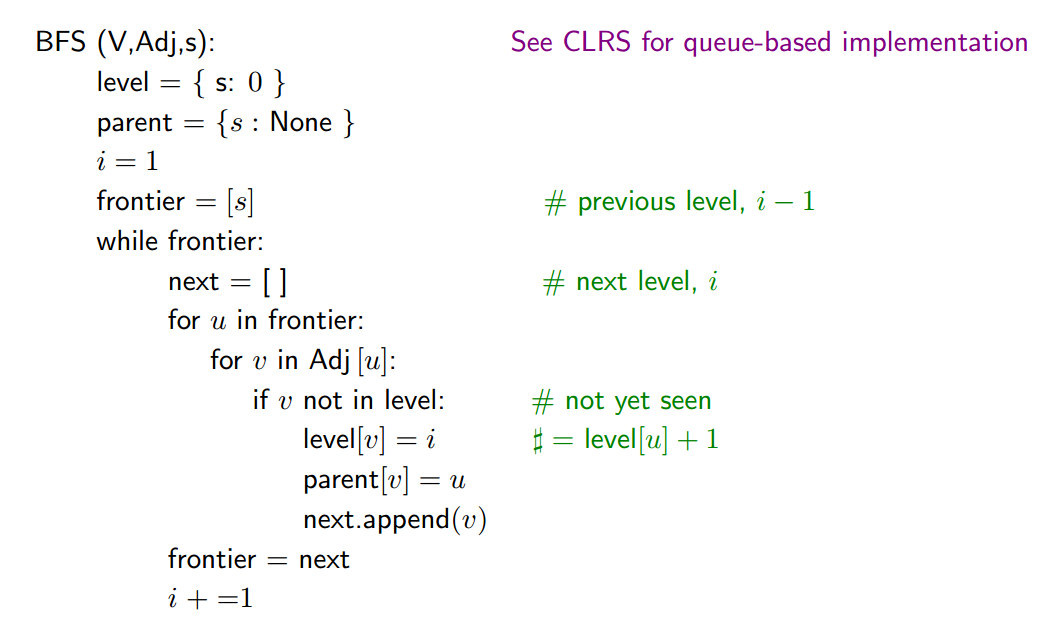
\includegraphics[scale=0.3]{bfs}

\section{DFS}
\begin{verbatim}
visited = {}

def do_something(node):
    print node

def dfs_visit(node):
    visited[node] = True
    for child in graph[node]:
        if not child in visited:
            dfs_visit(child)
    do_something(node)

for node in graph.keys():
    if not node in visited:
        dfs_visit(node)
\end{verbatim}
The output reversed is also toposorted.

\section{SSSP}
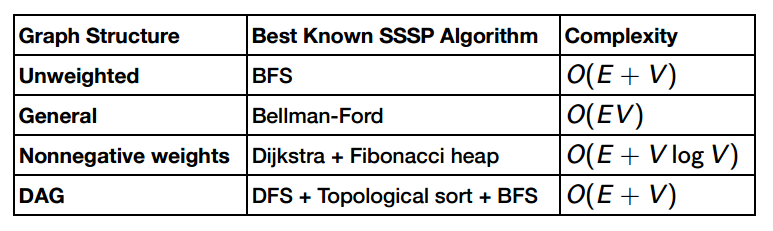
\includegraphics[scale=0.3]{sssp_summary}

\section{APSP}
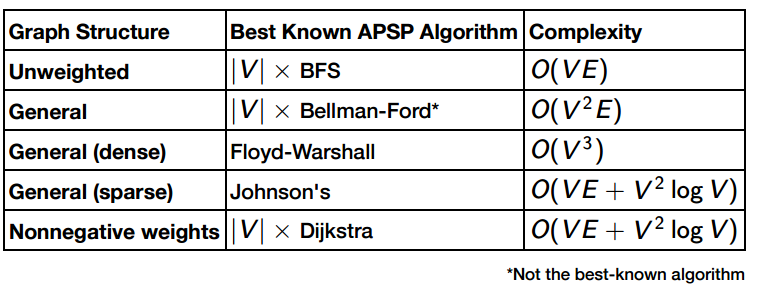
\includegraphics[scale=0.3]{apsp_summary}

\section{Dijkstra}
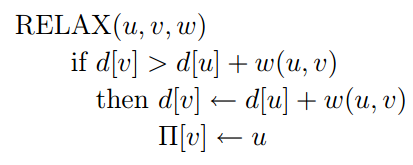
\includegraphics[scale=0.3]{relax}
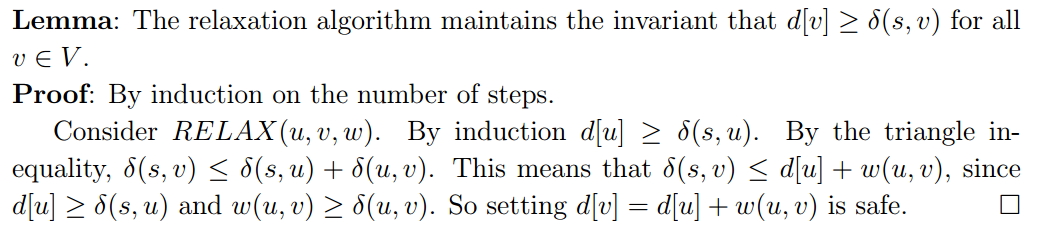
\includegraphics[scale=0.3]{relax_safe} \\

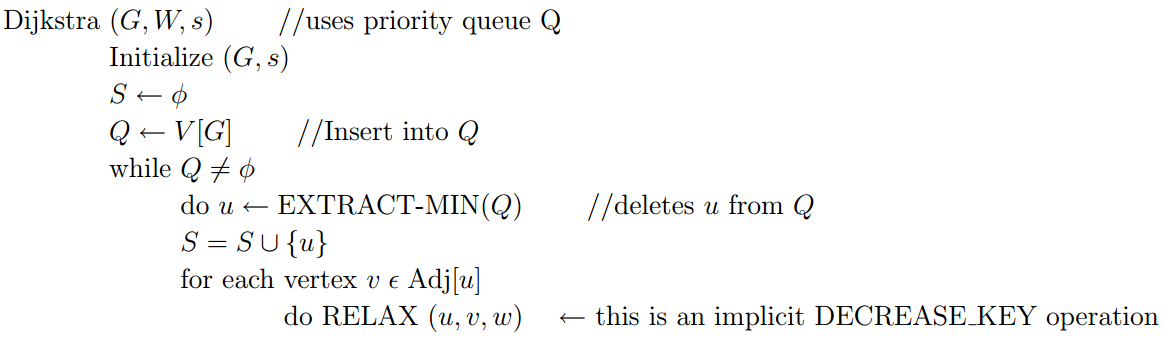
\includegraphics[scale=0.25]{dijkstra}

\section{Types of Edges}
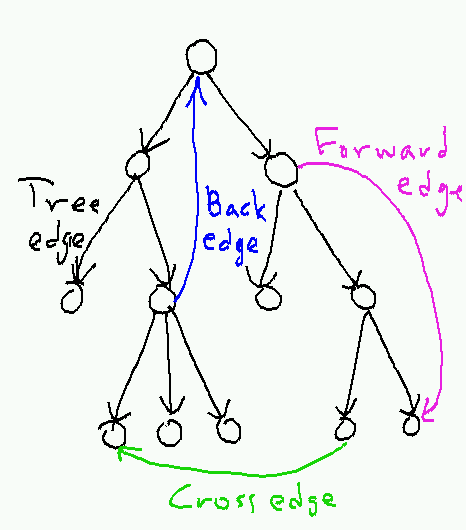
\includegraphics[scale=0.3]{edge_types.png}
\subsection{Proof That Difference of 1 is balanced}
$N_h$ is the minimum number of nodes that's possible of height $h$. Since the two sub trees differ by height 1,
\begin{align*}
N_h = 1 + N_{h-1} + N_{h-2} \\
> 1 + 2 N_{h-2} \\
> 2 N_{h-2} \\
= \Theta(2^{n/2}) \\
\implies h < 2 \log n
\end{align*}

\section{Open Addressing}
\subsection{Linear Probing}
Let's say you have a table with a cluster. If $h(k, i)$ maps to this cluster. At the end, you just increase your cluster length by 1. If $0.01 < \alpha = n/m < 0.99$ cluster are of size $\Theta(\ln n)$. Dict is not constant time any more.

\subsection{Double Hashing}
$h(k,i) = (h_i(k) + i h_2(k)) mod m$ if $h_2(k)$ is relatively prime $\implies$ permutation. Number of expected probes on operation insert $\leq \frac{1}{1 - \alpha}$ \\




\rule{0.3\linewidth}{0.25pt}
\scriptsize

Copyright \copyright\ 2014 Winston Chang

\href{http://www.stdout.org/~winston/latex/}{http://www.stdout.org/$\sim$winston/latex/}


\end{multicols}
\end{document}
